
% ----------------------------------------------------------
% Introdução
% ----------------------------------------------------------
\chapter{Introduction}
\label{sec:intro}

\gls{js} is one of the most popular programming languages
today~\cite{stackify,redmonk-javascript}, with penetration in various software development segments including, web, mobile,
and, more recently, the Internet of
Things~(IoT)~\cite{simply-technologies} and Machine Learning~\cite{github-ml}. The interest of the community
for the language encourages constant improvements in its specification~\cite{ecmas262-spec}. It is natural to expect that such improvements
lead to sensible changes in engine implementations~\cite{kangax}. Even small
changes can have high practical impact. For example, in October 2014 a
new attribute added to Array objects resulted in the MS Outlook
Calendar web app, which is built in \js{}, to fail under 
Chrome~\cite{array-bug-chromium-issue4247,array-bug-discussion}.

Finding bugs in \js\ engines is an important problem given the range
of applications that could be affected with those bugs. It is also
challenging.  Specifications are intentionally incomplete as to enable
development flexibility. In addition, they evolve frequently to
accommodate the pressing demands from
developers~\cite{ecmas262-spec-repo}. An official conformance test
suite exists for \js~\cite{tc39-github}, but, naturally, many test
scenarios are not covered in the suite. In addition, we noticed that a
significant fraction (5 to 15\%) of the tests fail regularly in the
most popular engines, reflecting the struggle of developers in keeping
up with the pace of spec evolution (see Table~\ref{tab:test262}).

%% WHAT WE DID
This work, which is empirical in nature, reports on a study to evaluate the importance of diversity
to find bugs in \js{} engines; it covers two complementary
diversity-aware testing techniques.

%\vspace{-1ex}
%noitemsep,
\begin{itemize}[topsep=0pt,parsep=0pt,partopsep=2pt,labelwidth=0cm,align=left,itemindent=-0.25cm]
\item \emph{Test transplantation} leverages diversity of test
  cases. This technique evaluates the effect of running test files
  written for a given engine in other engines. The intuition is that
  developers design test cases with different objectives in mind. As
  such, replaying these tests in different engines could reveal
  unanticipated problems.

\item \emph{Cross-engine differential testing} leverages diversity of
  engine implementations. This technique fuzzes existing test
  inputs~(\citeauthor{fuzz-testing-history}) and then compares the output
  produced by different engines.%\Comment{ using a differential oracle.}
  The intuition is that interesting inputs can be created
  from existing inputs and multiple engines can be used to address the
  lack of oracles.
\end{itemize}

The study measures the ability of these techniques in finding bugs and
the impact of \gls{fp} on their practicality.

%One of
%various causes of output discrepancy is a bug.

%% It automates test generation in scenarios where multiple
%% implementations of a system exist. DT leverages diversity across
%% system's implementations to detect anomalous behavior.
\emph{Related Ideas.}~The idea of test set diversity dates back to the
eighties~\cite{white-cohen-tse1980,ostrand-balcer-1988}. In contrast
to prior work on this topic, this study explores diversity of
implementations and diversity of sources of test cases as opposed to
diversity of the test cases themselves. Section~\ref{sec:related:diversity-testing}
elaborates related work on this topic. \gls{dt}~\cite{Brumley-etal-ss07}
has been applied in a variety of contexts to find
bugs~\cite{Yang-etal-pldi11,Chen-etal-fse2015,Argyros-etla-ccs16,Chen-etal-pldi16,petsios-etal-sp2017,SivakornAPKJ17,Zhang:2017:ATD:3097368.3097448}.
It has shown to be specially practical in scenarios where the
observation of difference gives a strong signal of a real problem. For
example, Mozilla runs JS files against different configurations of a
given build of their \smonkey\ engine (\eg{}, trying to enable or not
eager JIT compilation\footnote{These files are created with the
  grammar-based fuzzer jsfunfuzz~\cite{jsfunfuzz}. Look for option
  ``compare\_jit'' from funfuzz.}). A positive aspect of the approach
is that it can be fully automated---as only one engine is used, the
outcomes of the test in both configurations are expected to be
identical. The Mozilla team uses this approach since 2002; they have
been able to find over 270 bugs since
then~\cite{jsfunfuzz-at-mozilla}, including security
bugs. Cross-engine differential testing, in contrast, has not been
widely popularized. One possible reason is that it is still not
practical to fully automate the technique \Igor{due to the distinct
configurations of each engine, as well as a universal oracle
that would indicate possible true positives, this tasks still requires human
inspection}. In contrast to other
applications of differential testing, a number of legitimate reasons
exist, other than a bug, for a test execution to manifest discrepancy
(see Tables~\ref{fig:piecharts-transplantation} and~\ref{tab:false-positives}).
To sum up, variations of these ideas have
been explored before in different contexts.  The goal of the study is
to assess the ability of the techniques aforementioned in finding bugs
on \javascript\ engines.

%% This paper evaluates the benefits of
%% test case diversity and engine diversity in finding bugs on
%% \javascript\ engines.

%% Recently, Patra and
%% Pradel~\cite{patra2016learning} proposed a language-agnostic fuzzer to
%% find cross-browser HTML+JS discrepancies. The main difference of our
%% work to theirs is in goal; our goal is to evaluate ability and cost of
%% simple diversity-aware approaches to find bugs in \js\ engines.

%% Their main contribution was
%% analytical whereas our main contribution is empirical--

\begin{figure}[t]
%  \vspace{-2ex}  
  \centering
  \subfloat[\label{fig:stacked-engine}Bug reports per engine.]{
    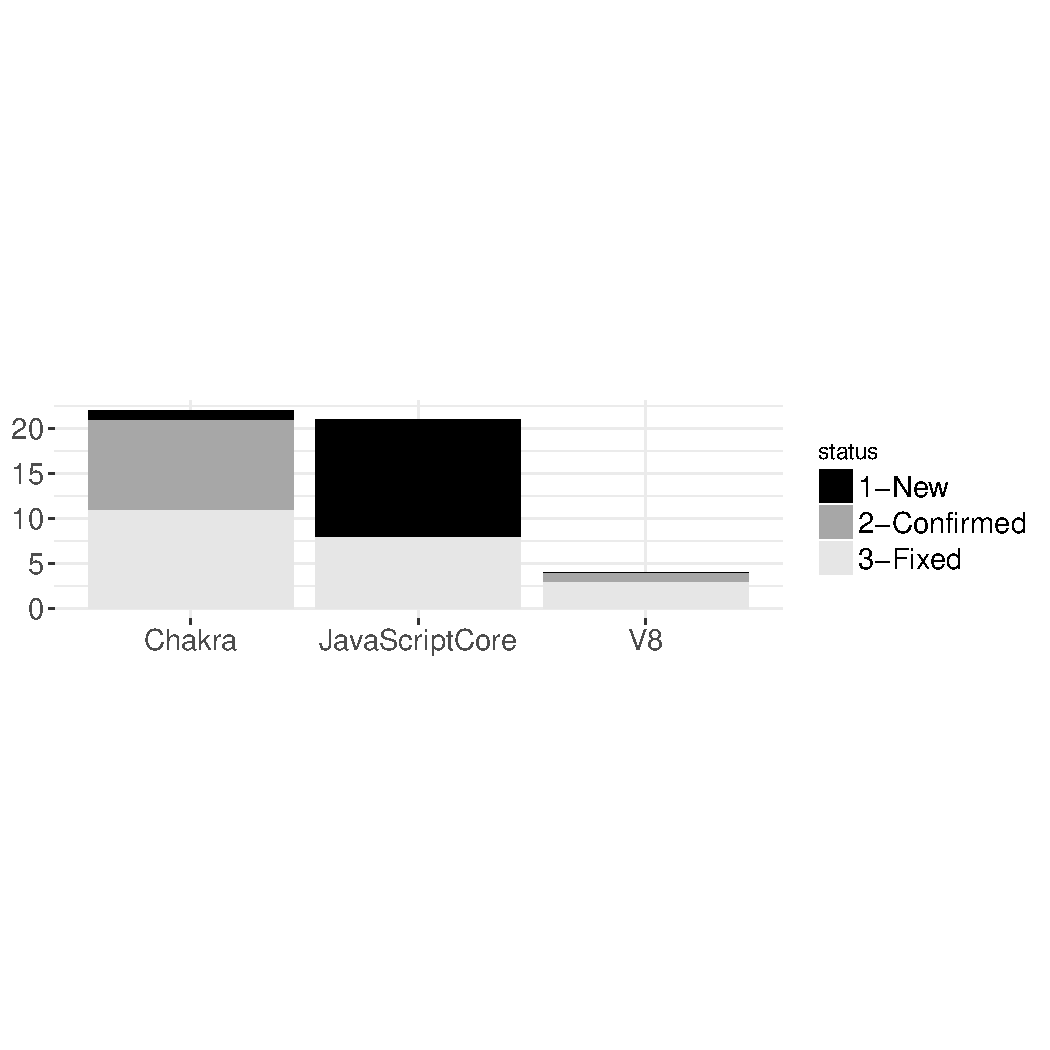
\includegraphics[trim=0 190 0 180,clip,width=0.7\textwidth,scale=0.4]{R/stackedbar/stacked-engine}
    \vspace{-5ex}
  }\\
  \subfloat[\label{fig:stacked-technique}Bugs reports per technique.]{
    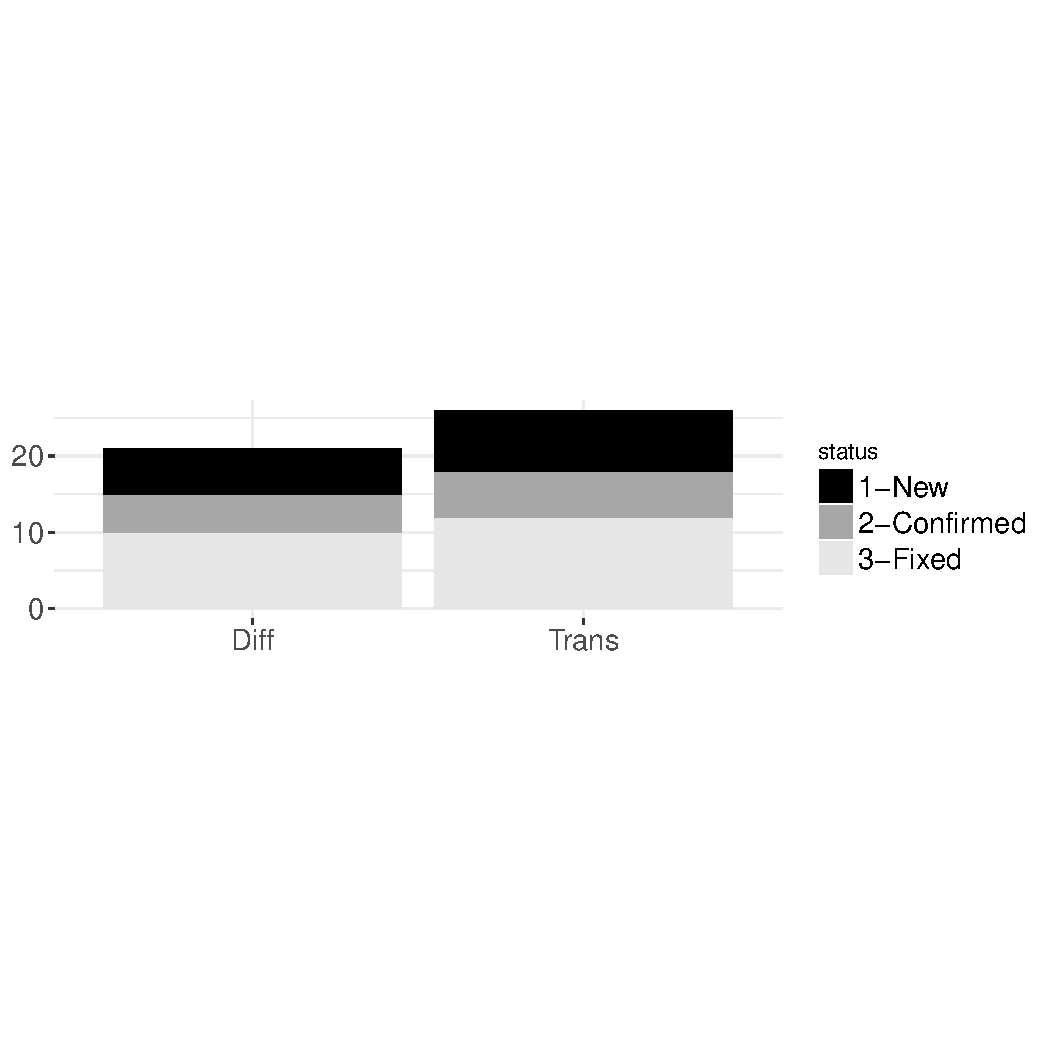
\includegraphics[trim=0 180 0 180,clip,width=0.7\textwidth,scale=0.4]{R/stackedbar/stacked-technique}
    \vspace{-5ex}        
  }
  \caption{\label{fig:summary}Summary of bug reports.}
  \vspace{-3ex}
\end{figure}

\sloppy \emph{Results.}~We considered the following engines--\chakra{}
(Microsoft), JavaScriptCore (Apple), \veight{} (Google), and
\smonkey{} (Mozilla). Figure~\ref{fig:summary} shows the breakdown of
bug reports per engine (\ref{fig:stacked-engine}) and per technique
(\ref{fig:stacked-technique}). Each stacked bar breaks down the bugs
per status (\eg{}, ``1-New''). The prefix number indicates the
ordering that status labels are assigned. Several of these
reports have the label ``3-Fixed'', indicating that bug fixes have
been incorporated into the code already. Note that most of these bugs
affected two engines--\chakra{} and JavaScriptCore (\jsc{}).  We
reported \noBugsBugsReportedGoogle{} bugs in \veight{}
(\noBugsBugsConfirmedGoogle{} confirmed) and none in \smonkey{}.
Furthermore, our results show that both techniques revealed several
bugs, most of which confirmed by developers. Test transplantation
revealed \noBugsTransplantation{} bugs (of which,
\noBugsTransplantationConfirmed{} were confirmed and
\noBugsTransplantationFixed{} were fixed) whereas differential testing
revealed \noBugsDifferentialTesting{} bugs (of which,
\noBugsDifferentialTestingConfirmed{} were confirmed and
\noBugsDifferentialTestingFixed{} were fixed).  Overall, results
indicate that both techniques were successful at finding bugs. The
number of bug reports were similar, if we consider only those
confirmed or fixed. Most bugs we found are of moderate severity.

%% Considering cost per bug found, we found that test
%% transplantation, compared to differential testing, demanded less
%% effort from the developers who inspected the alarms. 

%% All in all, these simple techniques
%% seem promising to improve reliability of engines that continuously
%% evolve with their specifications.

\emph{Key Findings.}~The list of findings of this work includes--1)
Not only multiple different implementations can be leveraged in
differential testing, but differences in test suites can also be
important. 2) Even for problems with fairly clear specifications, as
in \javascript{}, there is likely to be (a lot of) variation between
different implementations. 3) Differential testing is feasible on
real, complex, widely used pieces of
software. The Chapter~\ref{sec:lessons} expands and elaborates key
findings and lessons learned.

%% LIST OF CONTRIBUTIONS
\emph{Contributions.}~The most important contribution of this work is empirical: 
we provide a comprehensive study analyzing the effectiveness of diversity-aware
techniques to find functional bugs in popular \javascript\ engines.
Additional contributions are:
1)~A number of bugs found and fixed. 
We reported a total of \totalBugsReported{} bugs. 
Of these, \totalBugsConfirmed{} bugs were confirmed and \totalBugsFixed{} bugs were fixed. 
2)~An infrastructure for diversity-aware testing.
The scripts to run the experiments and the data are publicly available on our repository.
% \dataRepo{}.

\vspace{1ex} To summarize, this study provides initial, yet strong evidence
that exploring diversity should be encouraged to find functional bugs
in \js{} engines. 
 


% \lipsum[4]

% \begin{quadro}
% \caption{Caption do quadro}
% \label{quadro_modelo}
% \centering
% \begin{tabular}{|lllll|}
% \cline{1-5}
% A& B &  C& D &E  \\ \cline{1-5}
% \multirow{3}{*}{1}  & 2 &  3& 4& 5 \\
%  &  2 &  3& 4& 5  \\
%  &  2 &  3& 4& 5 \\
%  \cline{1-5}
% \end{tabular}
% \end{quadro}


% \begin{table}[]
%     \centering
%     \begin{tabular}{c|c}
%         f & b \\ \hline
%         2 & 3\\
%     \end{tabular}
%     \caption{tabela exemplo 1}
%     \label{tab:my_label}
% \end{table}

	
% \section{Overview of this thesis}

% \lipsum[4]
% \subsection{Publications}
% \lipsum[4]
% \section{Suport}

%  \gls{ddm},
% \gls{eddm}




% \begin{table}[ht]

%     \addtocounter{table}{-1}%<<<<<<
    
    % \begin{tabularx}{\linewidth}{@{}cX@{}}
    % \caption{Example of an table}\\
    % \toprule
    % \textbf{Column 1} & \textbf{Column 2} \\[6pt]
    % \midrule
    % \endhead
    % $R$ & 1This is an example sentence \\[6pt]
    % $R$ & 2As well as the line before \\[6pt]
    % $A$ & 3Also this is an example \\[6pt]
    % $R$ & 4This is an example sentence \\[6pt]
    % $R$ & 5As well as the line before \\[6pt]
    % $A$ & 6Also this is an example \\[6pt]
    % $R$ & 7This is an example sentence \\[6pt]
    % $R$ & 8As well as the line before \\[6pt]
    % $A$ & 9Also this is an example \\[6pt]
    % $R$ & 10This is an example sentence \\[6pt]
    % $R$ & 11As well as the line before \\[6pt]
    % $A$ & 12Also this is an example \\[6pt]
    % $R$ & 13This is an example sentence \\[6pt]
    % $R$ & 14As well as the line before \\[6pt]
    % $A$ & 15Also this is an example \\[6pt]
    % $R$ & 16This is an example sentence \\[6pt]
    % $R$ & 17As well as the line before \\[6pt]
    % $A$ & 18Also this is an example \\[6pt]
    % $R$ & 19This is an example sentence \\[6pt]
    % $R$ & 20As well as the line before \\[6pt]
    % $A$ & 21Also this is an example \\[6pt]
    % $R$ & 22This is an example sentence \\[6pt]
    % $R$ & 23As well as the line before \\[6pt]
    % $A$ & 24Also this is an example \\[6pt]
    % $R$ & 25This is an example sentence \\[6pt]
    % $R$ & 26As well as the line before \\[6pt]
    % $A$ & 27Also this is an example \\[6pt]
    % $R$ & 28This is an example sentence \\[6pt]
    % $R$ & 29As well as the line before \\[6pt]
    % $A$ & 30Also this is an example \\[6pt]
    % $R$ & 31This is an example sentence \\[6pt]
    % $R$ & 32As well as the line before \\[6pt]
    % $A$ & 33Also this is an example \\[6pt]
    % $R$ & 34This is an example sentence \\[6pt]
    % $R$ & 35As well as the line before \\[6pt]
    % $A$ & 36Also this is an example \\[6pt]
    % $R$ & 37This is an example sentence \\[6pt]
    % \bottomrule
    % \end{tabularx}

% \end{table}    
    
% \lipsum[4]
% \lipsum[4]
